Given a random variable $A$ and two real-valued functions $f$ and $g$ such that $X = f(A)$ and $Y = g(A)$ let $Z = h(X,Y)$ where $h$ is some real-value function from $\mathbb{R}^2$. The function $h(x,y) = x+y$ is of particular interest.

Since $A$ may be a mixed random variable the development will by assuming $A$ is discrete, then continuous and finally a general mixed random variable. In all cases $X$ and $Y$ are, by design, 100\% correlated through $A$.

\subsection{Discrete Operations on Correlated Random Variables}

Suppose that,

\begin{align*}
A = ((a_1, a_2, ..., a_n), (p_1, p_2, ..., p_n))
\end{align*}

where $Pr[A = a_i] = p_i$ for any $i \in 1...n$, that is, $A$ is a discrete random variable. Consequently,

\begin{align*}
X = ((x_1, x_2, ..., x_n), (p_1, p_2, ..., p_n))\\
Y = ((y_1, y_2, ..., y_n), (p_1, p_2, ..., p_n))\\
\end{align*}

where $x_i = f(a_i)$ and $y_i = g(a_i)$  for each $i$. Notice that duplicate values of $x_i$ are possible. If it happens that $x_i < x_{i+1}$ for each $i \in 1...n-1$ then $X$ is said to be in \emph{proper form} and similarly for $A$ and $Y$. To emphasize that $X$ and $Y$ are derived in a pointwise order-preserving manner they may be written in \emph{synchronous} form,

\begin{align*}
X = (x_1, x_2, ..., x_n)\\
Y = (y_1, y_2, ..., y_n)
\end{align*}

where the probability values associated with each $x_i$ and $y_i$ are found in $A$. The joint probability distribution of $X$ and $Y$ is itself a random variable called $XY$. Stated in syncrhonous form,

\begin{align*}
XY = ((x_1, y_1), (x_2, y_2), ..., (x_n, y_n))
\end{align*}

A new random variable $Z = h(X,Y)$ is stated in synchronous form with respect to $A$ as,

\begin{align*}
Z &= (h(x_1, y_1), h(x_2, y_2), ..., h(x_n, y_n))
\end{align*}

To restate $Z$ in proper form requires two steps. The first is to remove duplicates form the range of $Z$,

\begin{align*}
\mathbf{R}(Z) = \{h(x_i, y_i)\}_{i \in 1..n}
\end{align*}

The second step is to find the probability associated with each element of the range of $Z$. Assuming the following proper form of $Z$ as,

\begin{align*}
Z = ((z_1, z_2, ..., z_m), (q_1, q_2, ..., q_m))
\end{align*}

where $m \le n$ then,

\begin{align*}
z_j &\in \mathbf{R}(Z) \text{, ordered ascending}\\
q_j &= \sum_{i | z_j = h(x_i, y_i)}p_i
\end{align*}

For example suppose,

\begin{align*}
A = ((a_1,a_2,a_3),(p_1,p_2,p_3))\\
X = (1,2,3)\\
Y = (1,3,2)
\end{align*}

The joint random variable $XY$ in synchronous form is,

\begin{align*}
XY = ((1,1), (2,3),(3,2))
\end{align*}

Suppose $Z = h(X,Y)$ where $h(x,y) = x+y$. Then $Z$ in synchronous form with respect to $A$ is,

\begin{align*}
Z = (2, 5, 5)
\end{align*}

To find the proper form of $Z$ the range is first determined,

\begin{align*}
\mathbf{R}(Z) = \{2,5\}
\end{align*}

the proper form of $Z$ is stated as,

\begin{align*}
Z = ((z_1, z_2), (q_1, q_2))
\end{align*}

where

\begin{align*}
q_1 &= p_1\\
q_2 &= p_2 + p_3
\end{align*}

since $Z = 5$ is the set $\{(x_2,y_2) = (2,3), (x_3, y_3) = (3,2)\}$. Notice that the process of finding $Z$ in proper form is that of integrating iso-value subsets of the joint $XY$ range, the domain of $Z$. 

\subsection{Continous Operations on Correlated Random Variables}

Suppose $A$ is a real-valued continous random variable. Let $P$ be the probability density function associate with $A$ and write $A \sim P$. The random variables $X = f(A)$ and $Y = g(A)$, in synchronous form, share this association with $A$, that is, $X ~ P$ and $Y ~ P$ for any real valued functions $f$ and $g$. The joint random variable $XY$ is also stated in synchronous form as $XY \sim P$. Finally, $Z = h(XY)$ for any real-valued function $h$ from $\mathbb{R}^2$ is also stated in synchronous form as $Z \sim P$. 

To form an interesting example consider that $X = f(A)$ and $Y = g(A)$ form a parametric curve in $XY$-space and that the probability density $P$ is distributed along this curve. If $Z = h(XY)$ such that $h(x,y) = x+y$ then iso-value contours in $XY$-space appear as parallel lines with slope $-1$. In the figure \ref{fig:XY_continous} the disjoint curves are the single parametric $(X,Y)$ curve and the dotted diagonal lines are the iso-value contours for addition of $X$ and $Y$. The probability density $P$ of $A$ would appear in the figure perpendicular to the $XY$ plane over the paremetric curve of $(X,Y$). From the figure it is apparent that $Pr(1 < Z < 5) = 1$. Notice that the iso-value contour labeled $5$ in the figure intersects the $XY$ curve at three places so that $Pr(Z = 4)$ is found as the sum of three probability density values in $P$. 

\begin{figure}
  \centering
  \includegraphics{Images/XY_continous.eps}
  \caption[Joint distribution of correlated Continuous $X$ and $Y$ in $XY$-space]
          {Distribution of Continuous $XY$}
  \label{fig:XY_continous}
\end{figure}

Stating the synchronous form of $Z$ with respect to $A$ is as simple as for $X$ and $Y$, that is, $Z \sim P$. Finding the proper form of $Z$ may be a more challenging problem. The procedure for computing a numerical approximation to the proper form of $Z$ is detailed in the dissertation \cite{fielden12}. Notice in particular that computing the proper form of a random variable may be avoided until and observation is required for reasons such as graphing or comparison to unrelated random variables and constant values.

\subsection{Mixed Discrete / Continuous Operations on Correlated Random Variables}

To prepare for the computation of operations on a pair of mixed discrete/continuous random variables dependent on a single common random variable, it is useful to develop the case where one operand is discrete and the other is continuous. This situation can only arise if $A$ is not a purely discrete random variable.

Suppose that $A$ is a continuous random variable such that $A \sim P$ as above. Suppose without loss of generality that $X$ is a discrete random variable and that $Y$ is a continuous random variable. A visual example of a possible joint random variable $XY$ appears in figure \ref{fig:XY_discrete_continuous}. Included in the figure are the iso-value contours used to compute $Z = h(XY)$ where $h(x,y) = x+y$ as the previous continous example. Notice that this case is not fundamentally different from the previous case where $X$ and $Y$ are both continous. In the figure $X$ has four unique values in its range labeled $x_1, x_2, x_3, x_4$. It is apparent from the figure that $Pr(1 < Z < 5) = 1$ and that $Z$ is a continuous random variable. The procedure for computing a numerical approximation to the proper form of $Z$ is detailed in the dissertation \cite{fielden12}. 

\begin{figure}
  \centering
  \includegraphics{Images/XY_discrete_continous.eps}
  \caption[Joint Distribution of Correlated Discrete $X$ and Continous $Y$ in $XY$-space]
          {Distribution of Discrete/Continous $XY$}
  \label{fig:XY_discrete_continuous}
\end{figure}

\subsection{Operations on Correlated Mixed Random Variables}

If random variable $A$ is \emph{mixed}, that is, containing both continous and discrete probability distributions it is useful to decompose it into discrete and continous components and write,

\begin{align*}
A = A_d \oplus A_c
\end{align*}

where $A_d$ is a discrete random variable and $A_c$ is a continuous random variable and the $'\oplus'$ operator performs a sum of distribution functions by converting discrete probability to Dirac Delta functions. The components of $A$ are written as,

\begin{align*}
A_d &= ((a_1, ..., a_n),(p_1, ..., p_n))\\
A_c &\sim Q
\end{align*}

where $Q$ is a conditional probability distribution represented by a continuous probability density function. Notice that if $d = Pr(A_d)$ then $Pr(A_c) = 1-d$. That is,

\begin{align*}
d &= \sum_{i = 1..n}p_i\\
1-d &= \int_{A_c} dQ
\end{align*}

where the abuse of integral notation implies that the integral is performed over the range of $A_c$ in the usual sense. A non-trivial mixed random variable then requires that $0 < d < 1$. 

Notice in particular that for special case of addition of correlated random variables the operation of addition as in $Z = X+Y$ is that of projecting the $XY$ distribution to the diagonal as shown in figure \ref{fig:XY_addition_projection}. 

\begin{figure}
  \centering
  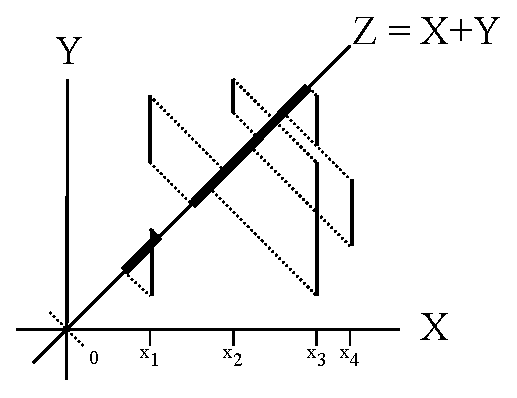
\includegraphics{Images/XY_addition_projection.eps}
  \caption[Projection of $XY$-space to $X+Y$-space]
          {Projection of $XY$-space to $X+Y$-space}
  \label{fig:XY_addition_projection}
\end{figure}

As an example suppose,

\begin{align*}
A &= \mathbf{U}(-1,2)\\
f(x) &= step(x) = \begin{cases}
0 & \text{ if x $\le$ 0},\\
1 & \text{ else}
\end{cases}\\
g(y) &= |y| + 1\\
X &= f(A)\\
Y &= g(A)
\end{align*}

then in proper form,

\begin{align*}
X &= ((0,1),(\frac{1}{3},\frac{2}{3}))\\
Y &= \mathbf{U}((0,1,2),(\frac{2}{3}, \frac{1}{3}))
\end{align*}

where $Y$ is \emph{multi-uniform} requiring probabilities within partition elements to be specified. Notice that $Pr(X = 0) = \frac{1}{3}$, $Pr(X = 1) = \frac{2}{3}$, $Pr(0 < Y < 1) = \frac{2}{3}$ and $Pr(1 < Y < 2) = \frac{1}{3}$. 

Suppose further that $Z = X+Y$. The joint $XY$ figure \ref{fig:XY_01_example} reveals the details. Noticing that the probability is uniformly distributed over the range of $XY$ and that the two fragments of that region do not overlap according to the iso-value contours of $Z$ the problem is solved by inspection so that,

\begin{align*}
Z \sim \mathbf{U}(1,4)
\end{align*}

\begin{figure}
  \centering
  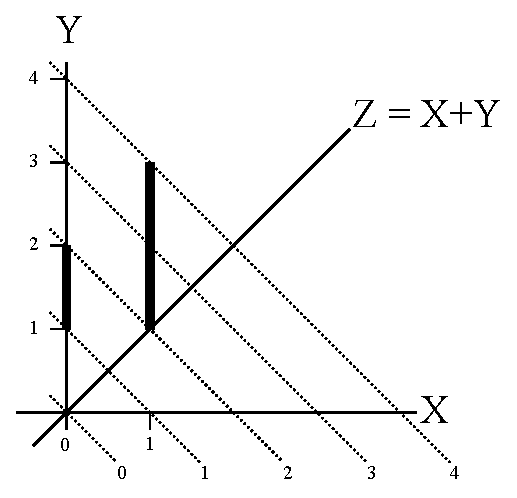
\includegraphics{Images/XY_01_example.eps}
  \caption[Example of Correlated Discrete $X$ and Continous $Y$ in $XY$-space]
          {Example of Discrete/Continous $XY$}
  \label{fig:XY_01_example}
\end{figure}

To find this result more formally $Y$ is conditioned on the discrete $X$ so that,

\begin{align*}
Y | X = 0 &\sim \mathbb{U}(1,2)\\
Y | X = 1 &\sim \mathbb{U}(1,3)
\end{align*}

then,

\begin{align*}
Z &= X + Y\\
  &= (X + Y | X = 0) \oplus (X + Y | X = 1)\\
  &= (0 + Y | X = 0) \oplus (1 + Y | X = 1)\\
  &\sim \mathbf{U}(1+0,2+0) * Pr(X = 0) + \mathbf{U}(1+1,3+1) * Pr(X = 1)\\
  &\sim \mathbf{U}(1,2) * \frac{1}{3} + \mathbf{U}(2,4) * \frac{2}{3}\\
  &\sim \mathbf{U}(1,4)
\end{align*}

For visual convenience the proper form distributions of $A$, $X$, $Y$ and $Z$ are shown in figure \ref{fig:XY_example_distributions}. Notice that to compute $Z = X + Y$ from the proper forms of $X$ and $Y$ is more challenging than from the synchronous form of $XY$ in figure \ref{fig:XY_01_example} in part because of the otherwise unseen correlation between $X$ and $Y$ through $A$.

\begin{figure}
  \centering
  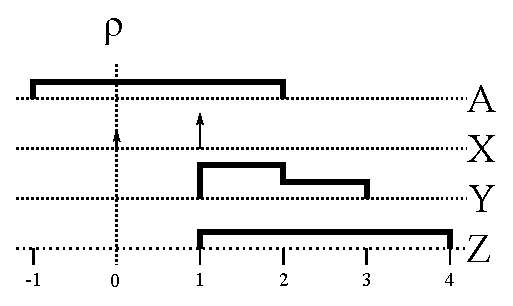
\includegraphics{Images/XY_example_distributions.eps}
  \caption[Example Discrete/Continuous Distributions in Proper Form]
          {Example Discrete/Continous Distributions in Proper Form}
  \label{fig:XY_example_distributions}
\end{figure}
